\chapter{Wstęp}

Rzeczywistość otaczająca człowieka i~jej aspekty są bardzo złożonym zagadnieniem. Człowiek w~procesie jej poznawania może postawić się w~różnych punktach odniesienia. Może obserwować rzeczywistość w~skali wszechświata badając i~poszerzając wiedzę na temat galaktyk oraz innych ciał niebieskich, gdzie Ziemia jest pomijalnie małym elementem. Może również obserwować świat w~skali makro i~mikroskopowej skupiając się na organizmach zamieszkujących i~strukturach budujących planetę, schodząc również na poziom atomów i~kwarków. 

Większość obserwacji nie może być dokonana bezpośrednio przez człowieka. Nie może on bowiem objąć wzrokiem całek galaktyki, albo dostrzec poszczególnych atomów. Obrazowanie takich zjawisk musi być zaprezentowane w~formie przystępnej dla człowieka wizualizacji zbudowanej z~uwzględnieniem konkretnych aspektów danego przypadku. 

Dobrze zbudowana wizualizacja danych, jaką jest chociażby prosty wykres punktowy, pozwala na analizę danych w~lepszym stopniu i~łatwiejsze wyciągnięcie wniosków. Dobrze skonstruowana wizualizacja, w~przypadku prezentacji jej większemu gronu odbiorców, pozwala również na skuteczniejsze zainteresowanie grupy tematem oraz pomóc w~opowiedzeniu historii, a~co za tym idzie, na wyciągnięcie przez odbiorców właściwych wniosków \cite{StorytellingWithData}.

\section{Istota rzeczy}

Jednym z~obszarów, w~którym wizualizacje pełnią istotną rolę są reprezentacje zjawisk geograficznych oraz tych w~bliskim sąsiedztwie Ziemi. Prezentowane dane mogą być związane z~działalnością człowieka, bądź z~obiektami i~zjawiskami fizycznymi, którymi planeta się cechuje.

System, który zajmuje się wprowadzaniem, analizowaniem i~wizualizacją danych geograficznych jest nazywa się Systemem informacji geograficznej (ang. geographic information system, \textbf{GIS}). Może on wyświetlać informacje z~wielu źródeł ujęte w~warstwy, które wyświetlane razem w~różnych kombinacjach mogą nadawać danym różnego kontekstu. Każda wyświetlana informacja jest ściśle powiązana z~pozycją na powierzchni Ziemi. \cite[Rozdział 1.6]{IntroductionToHumanGeography}.

Wizualizacje danych mogą tyczyć się dowolnych zjawisk. GIS może obrazować podział terytorialny państw świata, jak i~położenie obiektów kosmicznych w~bliskim sąsiedztwie Ziemi. Korzystając z~aktualizowanych na bieżąco źródeł danych wizualizacje mogą obrazować zjawiska zmienne, pokazywać stan obecny, przeszły (Rysunek \ref{fig:c1_windy}), jak i~prognozować przyszłość. 

\begin{figure}[h]
    \centering
    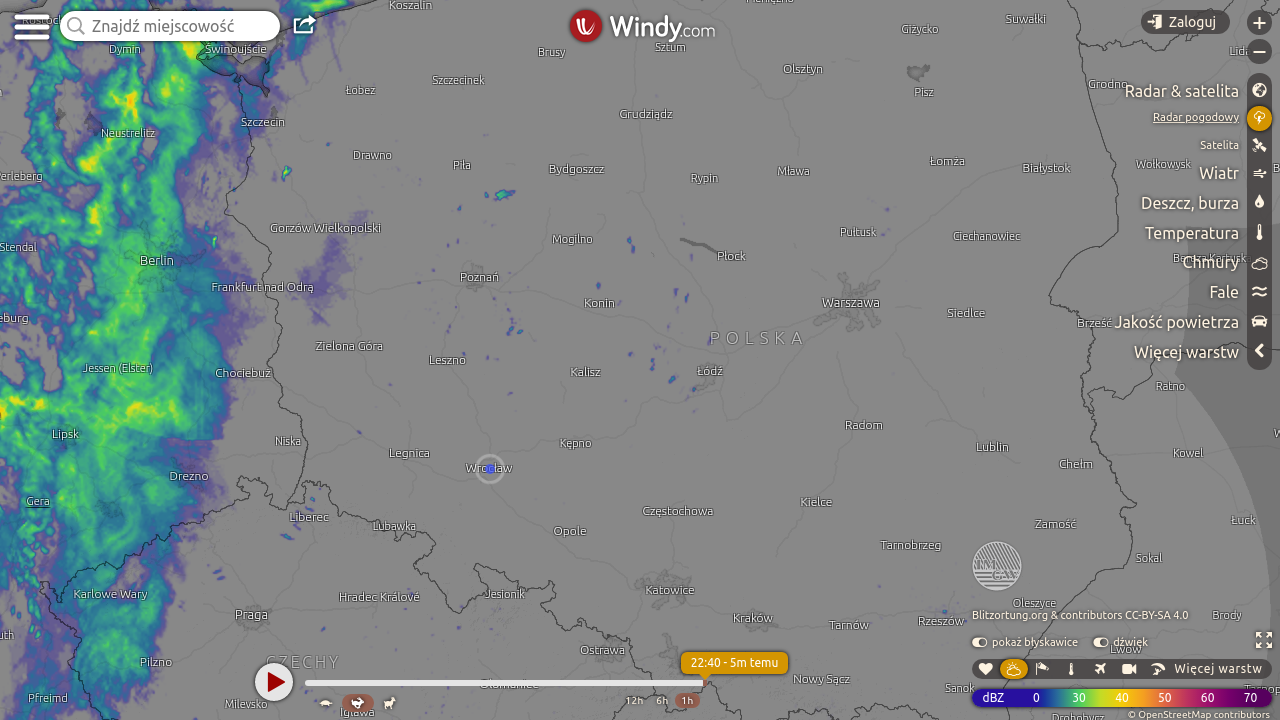
\includegraphics[width=\linewidth]{img/c1_windy.png}
    \caption{Widok wizualizacji dwuwymiarowej na stronie \textit{windy.com} wyświetlający informacje pogodowe na dwuwymiarowej mapie}
    \label{fig:c1_windy}
\end{figure}

Ważnym czynnikiem odbiorze wizualizacji, jest jej przystępność dla użytkownika. Profesjonalne, skomplikowane systemy nierzadko cechują się złożonym interfejsem użytkownika. Duża liczba opcji pomaga łatwo uzyskać pożądane dane przez profesjonalnego użytkownika, ale odstraszyć może niezagłębionego w~temat odbiorcę. Przystępność odbioru wiąże się również z~szybkością uzyskania dostępu do samej platformy obsługującej wizualizację. Alternatywą dla instalowanych aplikacji desktopowych jest przeglądarka internetowa. Tworzy ona środowisko, które może być uruchomione na wielu systemach operacyjnych, również na urządzeniach mobilnych, a~zaimplementowane wspomaganie sprzętowe generowania grafiki i~interfejsy takie jak \textit{HTML5 Canvas}\cite{Canvas} i~\textit{WebGL}\cite{WebGL} czynią ją potężnym narzędziem do wydajnego wyświetlania złożonych grafik. 
Aplikacje webowe oczywiście nie będą nigdy dorównywać profesjonalnym aplikacjom dedykowanym konkretnej platformie, jednak stanowią ich dobrą i~ogólnodostępną alternatywę.

Innym kryterium definiującym wizualizację jest jej interaktywność. Definiuje ono w~jakim stopniu użytkownik może dostosować wyświetlany widok, zarządzać warstwami, sterować położeniem kamery, czy też wyszukiwać informacje. Dwuwymiarowy widok mapy (Rysunek \ref{fig:c1_windy}) pozwala jednoznacznie odnieść informacje z~różnych warstw do konkretnego miejsca na planecie. Z~kolej widok trójwymiarowy (Rysunek \ref{fig:c1_google_earth}) pozwala na obserwację sceny z~różnych perspektyw, pokazuje kulistość Ziemi i~redukuje efekty zniekształcenia danych związany z~techniką rzutowania sfery na płaszczyznę. Przy kamerze skierowanej prostopadle do płaszczyzny powierzchni, oraz w~bliskim powiększeniu widok taki jest porównywalny do widoku dwuwymiarowego. Czynniki te zdaniem autora pracy czynią taką wizualizację bardziej atrakcyjną dla ogólnego odbiorcy. Oczywiście wybór techniki wizualizacji zawsze zależy od konkretnego przypadku, jak i~od oczekiwanej wydajności, gdyż złożoność generowania grafiki w~przypadku wizualizacji trójwymiarowych jest z~reguły większa.


\begin{figure}[h]
    \centering
    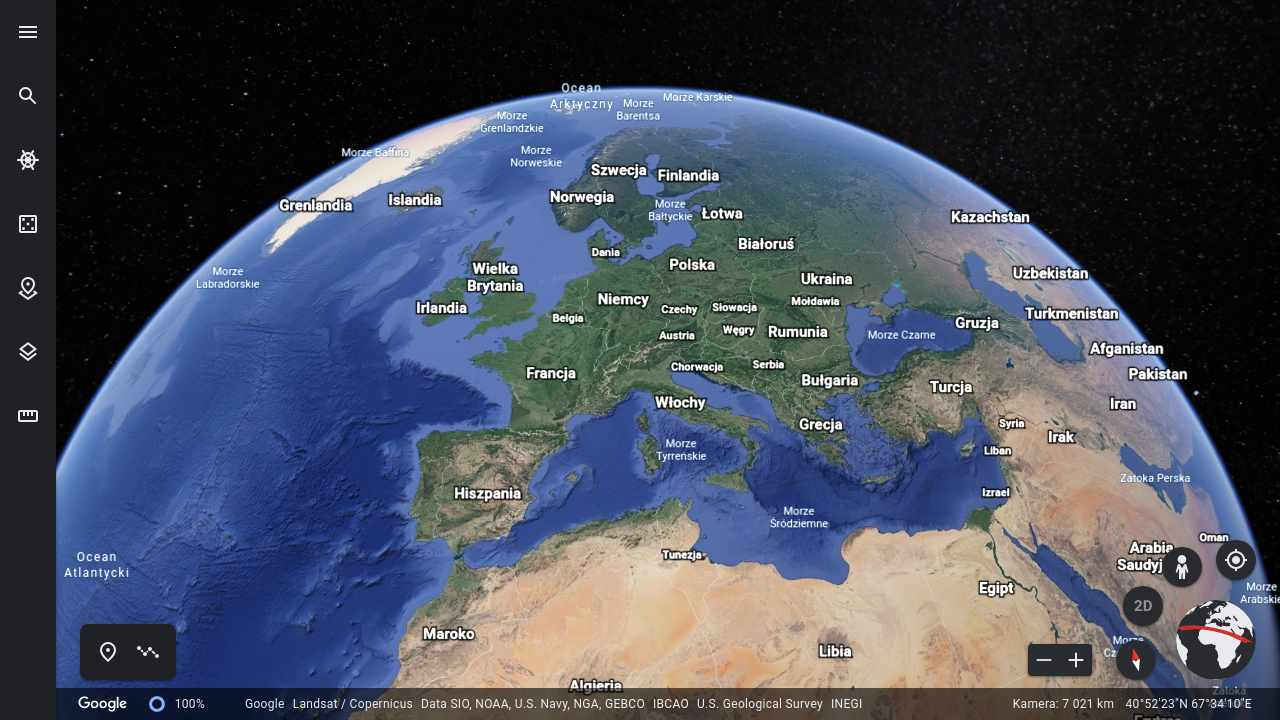
\includegraphics[width=\linewidth]{img/c1_google_earth.png}
    \caption{Widok wizualizacji trójwymiarowej na stronie \textit{earth.google.com}}
    \label{fig:c1_google_earth}
\end{figure}

\subsection{Podejścia do tworzenia wizualizacji}

Zadaniem twórcy wizualizacji jest zebranie i~przetworzenie danych na formę grafiki 2D lub 3D. Od używanego systemu informacji przestrzennej zależy w~jaki sposób definiowana jest wizualizacja i~skutkiem tego, jaki poziom wiedzy i~umiejętności z~danej dziedziny jest potrzebny do jej stworzenia. System w~definicji wizualizacji opiera się na swoich założeniach. Aplikacje uruchamiane bezpośrednio w~środowisku systemu operacyjnego mogą być wyposażone w~rozbudowane kreatory i~edytory, które zaspokajają wymagania użytkowników. Pozwalają skupić się na zagadnieniach domenowych, na poprawności i~dokładności wizualizacji zamiast na aspektach generowania grafiki. 

W środowisku przeglądarki internetowej do tworzenia wizualizacji nie stosuje się zwykle rozbudowanych edytorów graficznych i~formularzy. Biblioteki wyświetlające dane geoprzestrzenne konfigurowalne są zwykle z~poziomu języka JavaScript. Przykładem takiej biblioteki jest Cesium\cite{CesiumJS}. Potrafi ona generować wizualizacje 2D i~3D różnego rodzaju danych, a~jej konfiguracja następuje poprzez jej API, które dostarcza, ale też ogranicza jej możliwości (listing \ref{lst:cesium}).

\begin{lstlisting}[label={lst:cesium}, language=javascript, caption={Konfiguracja podstawowej wizualizacji w~bibliotece Cesium. Żródło: \url{https://cesium.com/docs/tutorials/getting-started/}}]
<script>
    Cesium.Ion.defaultAccessToken = 'your_access_token';
    var viewer = new Cesium.Viewer('cesiumContainer', {
        terrainProvider: Cesium.createWorldTerrain()
    });

    var tileset = viewer.scene.primitives.add(
        new Cesium.Cesium3DTileset({
            url: Cesium.IonResource.fromAssetId(your_asset_id)
        })
    );
    viewer.zoomTo(tileset);
</script>
\end{lstlisting}

Jeszcze innym podejściem, możliwym do zastosowania w~przypadku aplikacji i~desktopowych, i~webowych, jest dostarczenie twórcy tylko podstawowych abstrakcji (najczęściej interfejsów programistycznych) wizualizacji takich jak sterowanie kamerą, przekazywanie zdarzeń pochodzących od odbiorcy, czy interfejs służący do generowania obiektów na scenie 2D lub 3D. Podejście daje to najwięcej możliwości, ale z~drugiej strony wymaga posiadania największej wiedzy o~funkcjonowaniu dostarczonych interfejsów.

W każdym wypadku istotnym czynnikiem ułatwiającym tworzenie wizualizacji jest dostarczona przez narzędzia i~biblioteki interaktywna dokumentacja. Powinna ona dobrze opisywać dostarczone rozwiązania ze strony praktycznej i~przez swoją interaktywność ułatwiać poruszanie się po niej użytkownikowi. 

\section{Cel projektu i~zawartość pracy}

Celem opisywanego projektu jest stworzenie biblioteki umożliwiającej definiowanie i~wyświetlanie trójwymiarowych wizualizacji w~środowisku przeglądarki internetowej. Projekt zakłada również stworzenie aplikacji webowej, która za pomocą osadzonej w~niej, stworzonej biblioteki, umożliwia zarządzanie wyświetlaniem dostarczonych wizualizacji.

Rozdział drugi pracy opisuje szczegółowe wymagania postawione przed poszczególnymi komponentami aplikacji. Rozdział trzeci opisuje projekt i~implementację komponentu Silnika wyświetlającego wizualizację, a~rozdział czwarty przedstawia implementację przykładowych wizualizacji, które możliwe są do zdefiniowania korzystając z~interfejsów dostarczonych przez Silnik. W rozdziale piątym opisana jest Aplikacja korzystająca z~komponentu Silnika zbierająca wizualizacje i~umożliwiająca filtrowanie i~przełączanie się pomiędzy nimi. Rozdział szósty opisuje sposoby testowania zaimplementowanych rozwiązań, a~rozdział siódmy przedstawia używane w~projekcie biblioteki pomocnicze wraz z~ich krótkim opisem. Rozdział ósmy podsumowuje całość projektu i~zwraca uwagę na problemy napotkane podczas implementacji, możliwości optymalizacji i~alternatywne rozwiązania poruszanych wcześniej kwestii projektowych i~implementacyjnych.